%\documentclass[11pt,french]{article}
\documentclass[final]{cvpr}

\usepackage[utf8]{inputenc}
\usepackage[english]{babel}
\usepackage{fontenc}
\usepackage{amsfonts}
\usepackage{amsmath}
\usepackage{graphicx}
\usepackage{bbm}
\usepackage[a4paper, margin=1.2in]{geometry}
\usepackage{hyperref}

\renewcommand{\thesection}{\Roman{section}}

\newcommand{\HRule}{\rule{\linewidth}{0.5mm}}
\addto\captionsfrench{\renewcommand{\chaptername}{Partie}}

\begin{document}
	\title{Project proposal :\\On style transfer networks\\}
	\author{
		Ramzi Sofiane Dakhmouche, Farid Najar\\[0.2cm]
		Master Mathematics and Artificial Intelligence}
	\date{Octobre 2020}
	\makeatletter
	\begin{titlepage}
		\centering
		\textsc{\LARGE Institut de Mathématiques d'Orsay \\ Université Paris-Saclay}\\[4cm]
		\HRule \\
		{ \huge \bfseries \@title[2cm] }
		\begin{Large}
			\@author
		\end{Large}
		\HRule
		\vfill
		
\includegraphics[width=0.35\textwidth]{paris-saclay.png}
		\hfill
		
\includegraphics[width=0.35\textwidth, height=2.5cm]{imo.png}
		\pagebreak
		%\tableofcontents
		\pagebreak
	\end{titlepage}


	\section*{Motivation and problem definition}
	Being able to transfer the style of an artwork or more generally an artifact to another is an interesting task for the generation, creation, or design of new paintings, structures, or vehicles of a particular style or which satisfy a certain number of constraints. More specifically, the separation of content and style of natural images has been addressed in \cite{1} using convolutional neural networks (CNNs). More precisely, the feature space provided by a pre-trained CNN (described in \cite{2}) was used to introduce \emph{A Neural Algorithm of Artistic Style}, a new algorithm to perform image style transfer. We aim at thoroughly  studying this algorithm, efficiently implementing it then trying to obtain similar results with Generative Adversarial Networks(GANs). A generalization of the problem may have applications in Generative Design\cite{7} and music composition. We get help from the research done in this domain\cite{1}\cite{2}\cite{4}. You can see a demonstration in \hyperref[example]{figure 1}.
	
	\section*{Methodology} 
	We will firstly address the problem using convolutional neural networks. We will use the publicly available pre-trained CNN built in \cite{2}. Stochastic gradient descent will be used to approximate our problem, which can be expressed \cite{6} as:   
	\begin{multline*}
	x_{*} = argmin_{x^\prime} \sum_{l \in \mathcal{L}_{c}} {\sum_{k} {||f_{l, k}(x_{c}) - f_{l,k}(x^\prime)||^2 }}  \\
	+ \lambda \sum_{l \in \mathcal{L}_{c}} {\omega_{l} \sum_{i, j} {|f_{l,i}^T f_{l,j}(x_{s}) - f_{l,i}^T f_{l,j}(x^\prime)|}} 
	\end{multline*}
	where $f_{l,k}$ is the output $N_{l}$ dimensional feature map of the pre-trained CNN at the $l^{th}$ layer and $k^{th}$ filter, $x_{c}$ is the source (content) image, $x_{s}$ is the reference painting (style image), $\omega_{l}$ weights of the covariance of the feature maps $f_{l,.}$ (which measure the closeness of style) and $x_{*}$ is the produced image. For GANs, the previous formulation will be adapted (and potentially modified accordingly). 
	Concerning the data, we have access to two databases. Moreover, we will use Tensor Flow or PyTorch for the implementation.  	
	
	\section*{Evaluation}
	We plan to evaluate our results by comparing them to those found in \cite{1} and \cite{4}, and by comparing the results obtained using CNNs to those obtained by GANs. A basic evaluation could also be to visually evaluate a number of images. 
	%\pagebreak
	
	\begin{figure}
		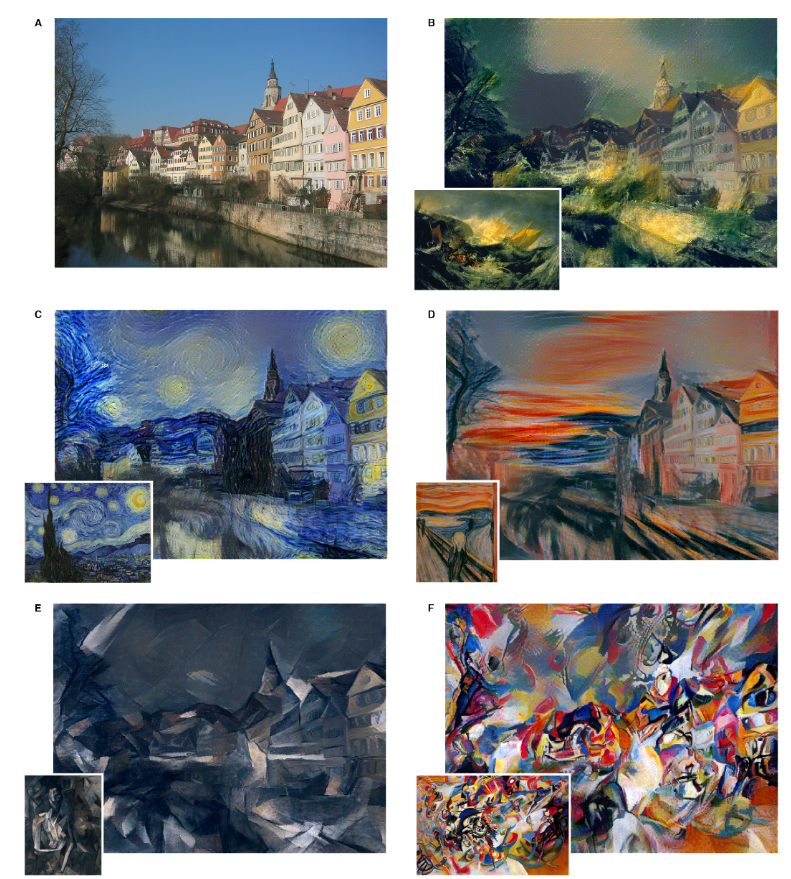
\includegraphics[width=.5\textwidth]{example.png}
		\label{example}
		\caption{The initial image A is transformed with respect to the painting given}
	\end{figure} 

	{\small
		\bibliographystyle{plain}
		\bibliography{biblio}
	}
        
\end{document}
